
%(BEGIN_QUESTION)
% Copyright 2006, Tony R. Kuphaldt, released under the Creative Commons Attribution License (v 1.0)
% This means you may do almost anything with this work of mine, so long as you give me proper credit

Determine the polarities of all voltage drops across all junctions made of dissimilar metal wires in the following thermocouple circuits:

$$\includegraphics[width=15.5cm]{i00375x01.eps}$$

$$\includegraphics[width=15.5cm]{i00375x02.eps}$$

\underbar{file i00375}
%(END_QUESTION)





%(BEGIN_ANSWER)

Hint: in order to answer this question, you are going to have to research what standard thermocouple types each dissimilar-metal junction forms, and the reference book(s) will tell you which metal is positive and which is negative.

$$\includegraphics[width=15.5cm]{i00375x03.eps}$$

$$\includegraphics[width=15.5cm]{i00375x04.eps}$$


%(END_ANSWER)





%(BEGIN_NOTES)

Polarities for the Constantan-Copper junctions may be found by researching type T thermocouples, which are made from unions of these two metals.  In a type T thermocouple junction, Copper is the positive (+) lead and Constantan is the negative ($-$).  The voltmeter's polarity is determined by means of Kirchhoff's Voltage Law: determining which Copper-Constantan junction produces more voltage (the hotter one, of course), and going with that.

We know the polarity of the iron-constantan junction by researching type J thermocouples.  We know the polarity of the copper-constantan junction by researching type T thermocouples.  We know the polarity of the iron-copper junction by experimentation (iron = + ; copper = -).

%INDEX% Measurement, temperature: thermocouple

%(END_NOTES)


